\chapter[Introdução]{Introdução}

\section{Justificativa}
Segundo o artigo 2$^{\circ}$ da legislação brasileira sobre pessoas com deficiência:
\begin{citacao}
Art. 2$^{\circ}$ Considera-se deficiência toda restrição física, intelectual ou sensorial, de natureza permanente ou transitória, que limita a capacidade de exercer uma ou mais atividades essenciais da vida diária e/ou atividades remuneradas, causada ou agravada pelo ambiente econômico e social, dificultando sua inclusão social.
\end{citacao}

De acordo com o senso de 2000 o Brasil tinha 14,5 \% da população com algum tipo de deficiência mental, auditiva, visual ou motora, desses 7\% possuem deficiência motora.  Pode-se observar na tabela \ref{tab:ibge} que há um aumento significativo de pessoas com deficiência motora na população de 65 anos ou mais de idade.

\begin{table}[ht!]
\centering
\caption{Distribuição percentual da população residente com deficiência motora segundo grupos de idade- Brasil-2010}
\begin{tabular}{|c|c|c|}
\hline
Grupos de idade & Total  & Deficiência Motora \\ \hline

Total           & 100,00 & 7,0                \\ \hline
0 - 14 anos       & 100,00 & 1,0                \\ \hline
15 - 64 anos    & 100,00 & 5,7                \\ \hline
65 anos ou mais & 100,00 & 38,3              \\ \hline

\end{tabular}
\legend{Fonte: \cite{censo_ibge} }
\label{tab:ibge}
\end{table}

As pessoas com deficiências motoras que pode decorrer de lesões neurológicas, neuromusculares, ortopédicas, mal formação e ainda amputação dos membros inferiores necessitam de cadeiras de rodas no seu dia-a-dia. A cadeira de rodas é imprescindível para permitir uma maior independência e qualidade de vida às pessoas com déficit de mobilidade. \cite{relatorio_sus}

Nos últimos anos cada vez mais se observa a luta pelo os direitos de pessoas com deficiência, nesse âmbito a lei n$^{\circ}$ 10.779, de 9 de março de 2001 obriga os ''"shopping centers"'' e estabelecimentos similares, em todo o Estado de São Paulo, a fornecer cadeiras de rodas para pessoas portadoras de deficiência e para idosos.

\subsection{Cadeira de Rodas Motorizadas}

As cadeiras de rodas motorizadas proporcionam conforto, segurança, rapidez e prevenção de lesões nos membros superiores devido ao uso repetitivo em cadeiras de rodas manuais. Entre tudo uma cadeira de rodas motorizada representa um alto custo. Em uma análise do impacto orçamentário realisada pelo Departamento de Economia da Saúde, Investimento e Desenvolvimento- Ministério da Saúde-DESID/SE/MS, o preço sugerido para uma cadeira de rodas motorizada é de R\$ 4.999,00, além do custo de manutenção. \cite{relatorio_sus}

Além disso, outro problema que as cadeiras de rodas motorizadas possuem é que em caso de necessidade não podem ser usadas como cadeiras de rodas manuais, pois possuem rodas pequenas para aproveitar melhor a potência dos motores e sistema de transmissão. Outro detalhe importante é que cadeiras de rodas motorizadas são geralmente pesadas, e não possuem as facilidades de transportes das cadeiras manuais.

\section{Estado técnico}

A evolução da cadeira de rodas motorizadas pode ser observada com a evolução de patentes relacionadas ao seu estado técnico. Parte desta evolução se passa em relação a estrutura da cadeira em si, uma vez que estas são melhoradas com o objetivo de se melhorar a estética e a ergonomia \cite{artigo_rudi}, esta evolução pode ser vista na figura \ref{fig:cadeiras_evolucao}

\begin{figure}[!htb]
\centering
  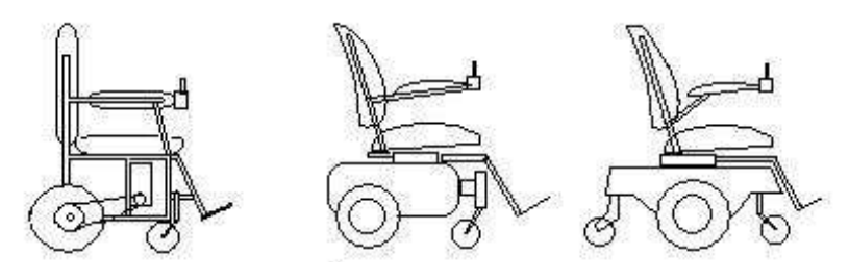
\includegraphics[keepaspectratio=true,scale=0.6]{figuras/introducao/cadeiras_evolucao}
\caption{Evolução das cadeiras motorizadas de 1971 a 1996}
\label{fig:cadeiras_evolucao}
\legend{Fonte: \cite[p.~2]{artigo_rudi}}
\end{figure}

A outra parte desta evolução se dá pela formalização de como a motorização do cadeira de rodas deva ser feita, uma vez que existem patentes relacionadas a tração: nas rodas da cadeira e de dispositivos que podem tanto empurrar como rebocar a cadeira \cite{artigo_rudi}. A figura \ref{fig:reboque} ilustra o dispostivo de reboque e a figura \ref{fig:anexo_empurrando} ilustra o dispostivo para empurar.

\begin{figure}[!htb]
\centering
  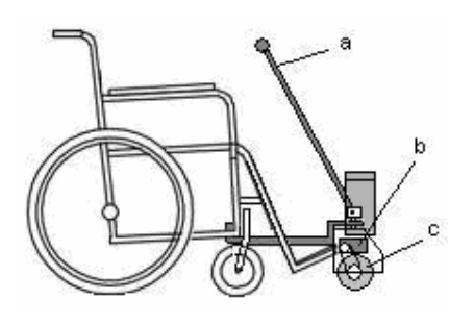
\includegraphics[keepaspectratio=true,scale=0.6]{figuras/introducao/reboque}
\caption{Dispositivo de reboque}
\label{fig:reboque}
\legend{Fonte: \cite[p.~3]{artigo_rudi}}
\end{figure}

\begin{figure}[!htb]
\centering
  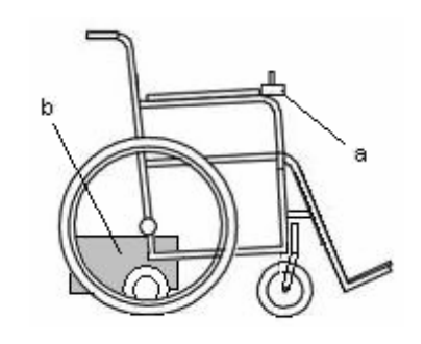
\includegraphics[keepaspectratio=true,scale=0.6]{figuras/introducao/anexo_empurrando}
\caption{Dispostivo para empurrar}
\label{fig:anexo_empurrando}
\legend{Fonte: \cite[p.~3]{artigo_rudi}}
\end{figure}

No artigo de \cite{artigo_rudi} também pode ser observado que:
\begin{citacao}
Quanto à utilização de cadeiras manuais adaptadas encontram-se algumas iniciativas na literatura científica e técnica. Todas apresentam diferentes formas de motorização da roda traseira, algumas utilizam correias [..] para
transmitir o movimento do motor [...] a uma polia conectada ao eixo de cada roda traseira [...] outras utilizam
correntes. Algumas fixam a polia à roda o que evita trabalho de adaptação do mancal existente na cadeira adaptada, mas isso dificulta a desmontagem para transporte.
\end{citacao}


\section{Objetivos}

Pretende-se projetar um sistema que possa ser acoplado a cadeiras de rodas manuais convencionais e transforma-las em cadeiras de rodas motorizadas. Visando o público alvo de shopping centers, com uma grande vantagem além do custo significantemente reduzido, a possibilidade do cadeirante de usufruir dos benefícios da cadeira motorizada sem perder a liberdade que o seu próprio modelo manual proporciona.
